% vim: nocindent:

\documentclass[ukrainian,utf8,pointsubsection,simple]{eskdtext}
%\documentclass[ukrainian,utf8,14pt]{extarticle}
\usepackage{pscyr}
\usepackage[utf8]{inputenc}
%\usepackage[cm]{fullpage}
%\usepackage[top=2in, bottom=1.5in, left=1in, right=1in]{geometry}
\usepackage[ukrainian]{babel}
\usepackage[T2A]{fontenc}
\usepackage{amsmath}
\usepackage{amssymb}
\usepackage{graphicx}
\usepackage{verbatim}
\usepackage{tabularx}
\usepackage{indentfirst}
\usepackage{lscape}
\usepackage{paralist}
\usepackage{gost}
\usepackage{longtable}
\usepackage[thmmarks,amsmath]{ntheorem}
\usepackage[unicode]{hyperref}


\ESKDsignature{IАЛЦ 467531.002 ПЗ}
\ESKDauthor{Радер Р.І.}
\ESKDchecker{Кулаков Ю.О.}
\ESKDtitle{\small{Система виявлення аномальної поведінки абонентів телефонної мережі}}
\ESKDdocName{Пояснювальна записка}
\ESKDgroup{НТУУ <<КПI>> \\ група IО-02}

\renewcommand{\labelenumi}{\arabic{enumi}. }


% Fit the abstract on a single page
% \ESKDsetPadding{7mm}{4mm}

% \newcommand{\abstracttile}[1]{%
% \begingroup%
% \centering\fontsize{18pt}{20pt}\selectfont\textbf{#1}\par%
% \endgroup}
\newcommand{\bignumberedpart}[1]{%
	\section{#1}
}
% \newcommand{\TBD}{
% 	TBD
% }

\begin{document}
\linespread{1.5}\selectfont

\newpage
\bignumberedpart{Охорона праці}
    В даній дипломній роботі була розроблена система для визначення аномальної поведінки абонентів телефонної мережі.

    Користувачем системи визначення аномальної поведінки є розробник цієї системи, співробітники оператора мобільного зв'язку або спеціалісти із технічної підтримки, які віддалено налаштовують та впроваджують систему. В обов'язки цих людей входить робота із мультикомп'ютерною системою віддалено за допомогою комп'ютерної мережі зі свого робочого місця, що облаштовано персональним комп'ютером. Умови праці випливають із робочого місця працівника.

    В даній роботі досліджена організація пожежної та електричної безпеки, параметри приміщень та вплив шкідливих та небезпечних факторів на працівників.
    
\subsection{Характеристика приміщення та умови його експлуатації}
    Програмний продукт, що розроблений в даній дипломній роботі, передбачається для використання спеціалістами із комп'ютерних систем та мереж. Робочі місця таких працівників розташоване у офісному приміщенні. План робочого приміщення приведений на рис.\ref{fig:lab-plan}.
    \begin{figure}[h!]
            \begin{center}
                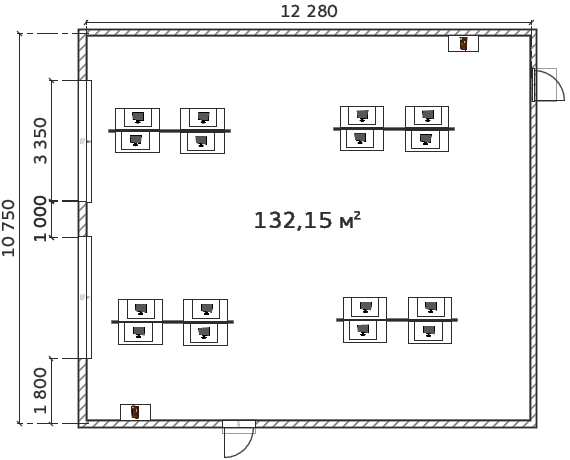
\includegraphics[scale=0.7]{labour/lab-plan.png}
            \end{center}
            \caption{Схема робочого приміщення}
            \label{fig:lab-plan}
    \end{figure}

    Геометричні параметри приміщення: ширина - 12.29 м, довжина - 10.75 м, висота - 3.5 м. Площа - 132.14 м кв., обєм - 462.49 м куб.
    У приміщенні передбачається розміщення 16 робочих місць обладнаних системними блоками та рідкокристалічними моніторами, живлення яких під'єднано до електричної мережі.

    Норматив ДНАОП 0.00-1.31-99\cite{lab-dnaop} передбачає на одного працюючого не менше 6 м кв. площі та не менше 20 м. куб. oб'єму.

    У офісному приміщенні, приведеному на рис.\ref{fig:lab-plan}, передбачено 16 робочих місць. Тоді відповідні параметри становлять 8.26 м. кв площі та при висоті стелі 3.5 м -  28.91 м куб. об'єму, що задовільняє норму.

    Для спрощення прокладки комунікацій стеля у приміщенні є підвісною. Для оздоблення стелі слід використовувати матеріали з коефіцієнтом відбиття 0.7 - 0.8, для стін 0.5 - 0.6.
    Покриття підлоги повинно бути матовим з коефіцієнтом відбиття 0.3 - 0.5. Поверхня підлоги повинна бути рівною і неслизькою.

    На робочому місці використовуються рідкокристалічні монітори (LCD) розміром 21 дюйм, які позбавлені багатьох недоліків (електромагнітне випромінювання, магнітне поле, мерехтіння і т.д.). На робочому місці присутній стіл глибиною 80 см, шириною 150 см та висотою 75 см від підлоги, присутній комп'ютерне крісло з можливістю налаштування висоти та регулювання кута наклону.

\subsection{Оцінка небезпечних і шкідливих виробничих факторів}
    \subsubsection{Мікрокліматичні умови}
    Категорія робіт, що виконуються на робочому місці є Іа - роботи, що виконуються сидячи і не потребують важкого фізичного навантаження ДСН 3.3.6.042-99\cite{lab-dsn42}. Роботи виконуються на постійному робочому місці.

    Мікроклімат у робочому приміщенні має відповідати наступним вимогам:
    \begin{itemize}
        \item оптимальна температура в холодний період року - 22..24 С, у теплий - 23..25 С;
        \item оптимальна відносна вологість 40-60\%;
        \item оптимальна швидкість руху повітря - 0.1 м/с;
        \item вміст шкідливих речовин у робочій зоні не повинен перевищувати ГДК.
    \end{itemize}

    Для підтримки оптимальної або допустимої температури в холодний період року приміщення повинно бути облаштоване системою водяного центрального опалення від місцевої або центральної теплової мережі, а в теплий період року - системою кондиціонування. Враховуючи, що у приміщенні встановлена підвісна стеля, може використовуватися спліт-система з внутрішнім блоком касетного типу.

    Вікна приміщення орієнтовані на північ, тому навіть у літній період не буде потрапляння прямих сонячних променів. Таке приміщення не потребує встановлення жалюзів на вікна.

    \subsubsection{Освітлення}

    На робочому місці проводяться зорові роботи із об'єктами 0.5 мм - 1 мм, контраст з об'єктів з фоном середній. Згідно з ДБН В.2.5-28-2006\cite{lab-dbn28} такий вид робіт відповідає розряду ІVг.

    Система освітлення у приміщенні суміщена, здійснюється як за допомогою природного світла з вікна, так і за рахунок штучних джерел на стелі. Сумарне освітлення робочої зони має бути таким, що сумарна освітленість на поверхні робочого столу становила 300 лк для розряду зорових робіт IVг (згідно ДБН В.2.5-28-2006\cite{lab-dbn28}).

    Природнє освітлення здійснюється за рахунок вікон орієнтованих на північ: два вікна, шириною 5 м та висотою 3 м. Загальна площа поверхні вікон 30 м кв.

    Штучне освітлення має здійснюватись переважно системою загального рівномірного освітлення. Рекомендованими є люмінесцентні лампи типу ЛБ - 32 лампи ЛБ-40 (цоколь G13) потужністю 40 Вт із застосуванням 8 світильників типу ЛВО 4х40 - світильник люмінісцентний, вбудований, для місць громадського користування на 4 лампи по 40 Вт кожна.
    Система загального освітлення повинна становити лінії світильників, розташованих збоку від робочих місць, паралельно лінії зору працюючих. План розміщення світильників штучного освітлення наведений на рис.\ref{fig:lab-plan-light}.

    \begin{figure}[h!]
            \begin{center}
                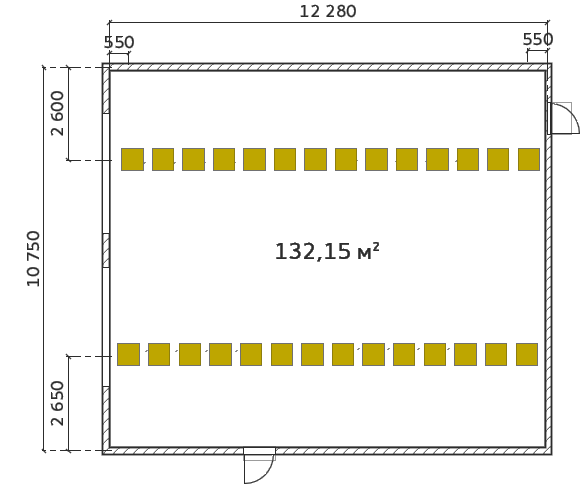
\includegraphics[scale=0.8]{labour/lab-plan-light.png}
            \end{center}
            \caption{Схема штучного освітлення робочого приміщення}
            \label{fig:lab-plan-light}
    \end{figure}

    Коефіцієнт природного освітлення (КПО) становить $e^{III}_n = 0.6$; відповідно
         до географічного розташування об'єкту у 4 поясі, коефіцієнт світлового клімату дорівнює $m = 0.9$, коефіцієнт сонячності клімату за умови що вікна орієнтовані на північ, а об'єкт росташований північніше 50 градусів, $C = 1.0$. Таким чином, нормативне значення природної освітленності
         становить:
         \[
             \textup{КПО} = e^{III} \cdot C \cdot m = 0.6 \cdot 0.9 \cdot 1.0 = 0,54
         \]

    Знайдемо площу вікон, що забеспечить нормоване значення КПО.

    \[
         S_B = \frac{S_{\textup{під}}}{100} \cdot \frac{e_n \cdot K_3 \cdot v_B \cdot K_{\textup{буд}}}{\tau \cdot r_1}
     \]

    Відношення довжини приміщення до його глибини $k_1 = \frac{10.75}{12.28} = 0,86$. Відношення глибини приміщення до висоти від рівня робочої поверхні до верхнього краю вікна $k_2 = \frac{12.28}{\frac{12.28}{3.5-0.75}} = 4,5$. Тоді світова характеристика вікон $v_B = 21$.

    $S_\textup{під} = 132,14 \textup{м}^2$ --- площа підлоги; $e_n = 0,81$ --- нормоване значення КПО; $ K_3 = 1,3$ --- коефіцієнт запасу; $ K_{\textup{буд}} = 1 $ --- коефіцієнт, що враховує
    затінення вікон будівлями, які розташовані навпроти; $\tau = 0,8 $ ---
    загальний коефіцієнт світопропускання; $r_1 = 1,2$ --- коефіцієнт, що
    враховує підвищення КПО при боковому освітленні завдяки світлу, яке
    відбивається від поверхонь приміщення (мінімальний). Підставляємо всі ці значення і
    отримуємо:
    \[
     S_B = \frac{132,14}{100} \cdot \frac{0,54 \cdot 1,3 \cdot 23 \cdot 1,0}{0,8 \cdot 1,2} = 29 \textup{м}^2
    \]

    Фактична площа більша ніж необхідна, тому природнє освітлення задовільняє норми.


        Розрахуємо відповідність штучного освітлення нормам. Для цього використаєм
        формулу світлового потоку:
        \[
            E_{\textup{ф}} = \frac{F_l \cdot N \cdot n \cdot \nu}{S_n \cdot K_3 \cdot Z}
        \],
        де  $F_{l}$ --- світловий потік однієї лампи в світильнику;
        $N$ --- кількість світильників; $n$ --- кількість ламп;
        $\nu$ --- коефіцієнт використання світлового потоку;
        $S_n$ --- площа приміщення; $K_3$ --- коефіцієнт запасу, розрахунковий
        коефіцієнт, що враховує зниження освітленності в процессі експлуатації
        внаслідок забруднення та старіння джерел світла, а також зниження
        показників відбиття поверхонь приміщення; $Z$ --- коефіцієнт нерівномірності
        освітлення.

        Показник приміщення за наступною формулою:
        \[
            i = \frac{ab}{h \cdot (a + b) = \frac{12,3 \cdot 10,75}{3,5 \cdot (12,3+10,75)}} = 1,63
        \]
        тоді коефіцієнт використання світового потоку становить $\nu = 58\% $.

        Світловий потік для використонуваних ламп становить 3200лм, а коефіціент
        нерівномірості 1.1

        Коефіцієнт запасу приймається рівним $K_3 = 1,3$.
        Підставляючи значення до основної формули методу світлового потоку отримаємо:
        \[
            E_{\textup{ф}} = \frac{3200 \cdot 8 \cdot 4 \cdot 0,58}{132,14 \cdot 1,3 \cdot 1.1} = 315 \textup{лм}
        \],
        що задовільняє норму в 300 лм.

    \subsubsection{Шум та вібрація}
    
        Згідно ДСН 3.3.6.037-99\cite{lab-dsn37} рівень шуму та рівні звукового тиску для програмістів та вчених (творчі професії), мають бути не більше 50 дБA. 

        Джерелами шуму є власний компютер та компьютери сусідів. Один комп'ютер з еквівалентим рівнем шуму одного - 40 дБА. Для пониження рівня шуму необхідно відрегулювати швидкість обертання кулерів центрального процесора та блоку живлення на допустимі значення. Це дозволяє знизити рівень шуму до 35 дБА.

        В одному блоку знаходиться 4 комп'ютера, сумарний шум $35 + 10lg(4) = 41$ дБА.
        В офісному приміщенні знаходяться 4 блоки, тому сумарний шум у приміщенні становить $$35 + 10lg(16) \approx 41 + 10lg(4) \approx 47 \textup{дБА}$$

        Отже, сумарний шум становить 47 дБА, що задовільняє норму 50 дБА.

        Вібрація на робочому місці не присутня.

    \subsubsection{Випромінювання}
    На робочому місці використовуються рідкокристалічні монітори (LCD), які позбавлені багатьох недоліків (електромагнітне випромінювання, магнітне поле, мерехтіння і т.д.).

    Рівні максимального електромагнітного випромінювання показані у таблиці \ref{tab:lab-waves}, причому максимальне значення
    електростатичного поля не повинно перевищувати 20 кВ/м.

    \begin{table}[h]
        \caption{Максимальні допустимі значення електромагнітного випромінювання на робочому місці}
        \begin{tabularx}{\textwidth}{| X | X | X |}
            \hline
            Частота електромагнітного поля (МГц) & Допустима напруженість (В/м) \\ \hline
            0.06 - 3     & 50                      \\ \hline
            3 - 30     & 20                      \\ \hline
            30 - 50    & 10                    \\ \hline
            50 - 300   & 5                      \\ \hline
        \end{tabularx}
        \label{tab:lab-waves}
    \end{table}

\subsection{Електрична безпека}
    У приміщенні характер виконуваних робіт пов'язаний з постійним використанням електроустановок(системних блоків, моніторів). Приміщення відноситься до класу без підвищеної небезпеки. Напруга у мережі становить 220В.

    Для забеспечення достатнього рівня електробезпеки, усі заземлені конструкції в приміщенні (батареї обігріву, водопровідні труби, кабелі з заземленим відкритим каналом), повинні бути захищені діелектричними щитками або сітками для недопущення потрапляння працівника під напругу. Для всієї проводки необхідно використовувати подвійну ізоляцію - основну та захисний короб.

    Необхідно забезпечити підключення заземлення всіх установок під напругою, обладнання в приміщенні повинно мати захист від короткого замикання та інших аварійних режимів, обладнання повинно підключатися виключно справними штепселями до стандартних електророзеток, лінія електромережі повинна бути окремою груповою трьохпроводною мережею, що складається з фазового, нульового робочого та нульового захисного провідників. Нульовий захисний провідник використовується для заземлення обладнання.

\subsection{Пожежна безпека}
    В приміщенні виконуються роботи із електричними установками, які можуть стати причиною пожежі. Забезпечення пожежної безпеки у приміщенні повинно здійснюватися комплексом заходів: організаційних, системи виявлення пожеж та системи пожежогасіння.
    До пожежонебезпечних матеріалів у розглянутому приміщенні можна віднести - тверді горючі речовини (дерев'яні меблі - столи, шафи), підісна стеля. Тоді згідно НАПБ Б.03.002-2007\cite{lab-napb} таке приміщення відноситься до категорії В(пожежонебезпечна).

    Потенційно можливі пожежі класу А -горіння твердих речовин, та класу Е - горіння електроустановок.

    Приміщення повинно відповідати вимогам системи попередження пожеж (максимальне використання негорючих матеріалів, застосування аварійного відключення на електроустановках, наявність систем виявлення пожежі, вогнегасників).

    Основні причини пожежі у приміщенні пов'язані з електричними приладами, напруга в яких не перевищує 380 В, необхідно встановити автоматичну дренчерну систему газового пожежогасіння з використанням хладона.

    Один димовий датчик контролює 30-50 м кв. Приміщення площею 132 м кв. має бути обладнане не менше ніж чотирма димовими датчиками сповіщення про пожежу.

\subsection{Техніка безпеки до виконання робіт}
    У приміщенні роботи проводяться з використанням пристроїв, що працюють під напругою: системні блоки, монітори. До виконання робіт допускаються виключно особи, що ознайомлені з усіма правилами безпеки.
    
    Виконання інструкцій техніки безпеки обов'язкове для всіх працівників.

    Перед початком робіт слід впевнитися, що у приміщенні немає проблем з електропроводкою. Заборонено починати роботи при наявності оголеної проводки.
    
    Заборонено включати електроприбори, якщо на робочому місці присутня волога(наприклад, розлита вода).
    
    Якщо під час включення комп'ютера виникли іскри або дим, слід негайно виключити електричний рубильник,
    при необхідності скористатися вогнегасником, та сповістити про це спеціальні служби.

    При потраплянні людини під напругу необхідно знеструмити відповідне робоче місце, надати першу долікарську допомогу і викликати «швидку».

    Не слід самостійно переключати будь-які запчастини, переєднувати проводи - це повинен робити фахівець.

    Не допускається наявність їжі та напоїв на робочому місці через загрози потрапляння води до електричних мереж.


\bibliographystyle{gost71s}
\bibliography{myrefs}


\end{document}
